%\documentclass[12pt,modern,twocolumn,tighten]{aastex63}
\documentclass[12pt,modern,tighten]{aastex63}
%\documentclass[12pt,modern,twocolumn,tighten,linenumbers,trackchanges]{aastex63}
%\documentclass[12pt,twocolumn,tighten,linenumbers]{aastex63}
%\documentclass[12pt,twocolumn,tighten,trackchanges]{aastex63}
\usepackage{amsmath,amstext,amssymb}
\usepackage[T1]{fontenc}
\usepackage{apjfonts}
\usepackage[figure,figure*]{hypcap}
\usepackage{graphics,graphicx}
\usepackage{hyperref}
\usepackage{natbib}
\usepackage[caption=false]{subfig} % for subfloat
\usepackage{enumitem} % for specific spacing of enumerate
\usepackage{epigraph}

\renewcommand*{\sectionautorefname}{Section} %for \autoref
\renewcommand*{\subsectionautorefname}{Section} %for \autoref

\newcommand{\cn}{Cep-Her complex} % cluster name
\newcommand{\sysone}{Kepler-1627} % star system name (binary)
\newcommand{\stone}{Kepler-1627 A} % star system name (binary)
\newcommand{\plone}{Kepler-1627 Ab} % planet name
\newcommand{\systwo}{Kepler-1643} % star system name (binary)
\newcommand{\sttwo}{Kepler-1643} % star system name (binary)
\newcommand{\pltwo}{Kepler-1643 b} % planet name
\newcommand{\systhree}{KOI-7368} % star system name (binary)
\newcommand{\stthree}{KOI-7368} % star system name (binary)
\newcommand{\plthree}{KOI-7368 b} % planet name
\newcommand{\sysfour}{KOI-7913 } % star system name (binary)
\newcommand{\stfour}{KOI-7913 A} % star system name (binary)
\newcommand{\plfour}{KOI-7913 Ab} % planet name

\newcommand{\clusterage}{$38^{+6}_{-5}$\,Myr} % 

%
% Symbols
%
\newcommand{\kms}{\,km\,s$^{-1}$}
\newcommand{\ms}{\,m\,s$^{-1}$}
\newcommand{\bpmrpo}{(G_{\rm BP}-G_{\rm RP})_0}
\newcommand{\bpmrp}{G_{\rm BP}-G_{\rm RP}}

%% Reintroduced the \received and \accepted commands from AASTeX v5.2.
%% Add "Submitted to " argument.
\received{\today}
\revised{---}
\accepted{---}
%\submitjournal{AAS Journals}
\shorttitle{Kepler Mini-Neptunes in Cep-Her}

\begin{document}

\title{
  Three 38 Million Year Old Mini-Neptunes from Kepler, TESS, and Gaia
}

%\suppressAffiliations
%\NewPageAfterKeywords
\correspondingauthor{L.\,G.\,Bouma}
\email{bouma.luke@gmail.com}

\author[0000-0002-0514-5538]{L. G. Bouma}
\affiliation{Department of Astrophysical Sciences, Princeton University, 4 Ivy Lane, Princeton, NJ 08540, USA}

% Key authors:
% ... stellar rotation & the initial crossmatch
\author[0000-0002-2792-134X]{J. L. Curtis}
\affiliation{Department of Astronomy, Columbia University, 550 West 120th Street, New York, NY 10027, USA}
\affiliation{Department of Astrophysics, American Museum of Natural History, New York, NY 10024, USA}

% ... Kepler correlations
\author[0000-0003-1298-9699]{K. Masuda}
\affiliation{Department of Earth and Space Science, Osaka University, Osaka 560-0043, Japan}

% ... HIRES PI
\author{L. A. Hillenbrand}
\affiliation{Cahill Center for Astrophysics, California Institute of Technology, Pasadena, CA 91125, USA}

% ... RM fitting
\author[0000-0001-7409-5688]{G. Stefansson}
\affiliation{Department of Astrophysical Sciences, Princeton University, 4 Ivy Lane, Princeton, NJ 08540, USA}

%
% PFS Collaborators
%
\author[0000-0001-8638-0320]{A. W. Howard}
\affiliation{Cahill Center for Astrophysics, California Institute of Technology, Pasadena, CA 91125, USA}
%
\author[0000-0002-0531-1073]{H. Isaacson}
\affiliation{Astronomy Department, University of California, Berkeley,
CA 94720, USA}

%
% MUSCAT3 Collaborators
%
\author[0000-0001-8511-2981]{N. Narita}
\affiliation{Komaba Institute for Science, The University of Tokyo, Tokyo 153-8902, Japan}
\affiliation{Japan Science and Technology Agency, PRESTO, Tokyo 153-8902, Japan}
\affiliation{Astrobiology Center, Tokyo 181-8588, Japan}
\affiliation{Instituto de Astrof\'{i}sica de Canarias (IAC), 38205 La Laguna, Tenerife, Spain}

\author[0000-0002-4909-5763]{A. Fukui} % afukui@g.ecc.u-tokyo.ac.jp
\affiliation{Komaba Institute for Science, The University of Tokyo, Tokyo 153-8902, Japan}
\affiliation{Instituto de Astrof\'{i}sica de Canarias (IAC), 38205 La Laguna, Tenerife, Spain}

\author[0000-0002-5658-5971]{Masahiro Ikoma} % ikoma.masahiro@gmail.com
\affiliation{Division of Science, National Astronomical Observatory of Japan, Tokyo 181-8588, Japan}

\author[0000-0002-6510-0681]{M. Tamura} % motohide.tamura@nao.ac.jp
\affiliation{Department of Astronomy, University of Tokyo, Tokyo 113-0033, Japan}
\affiliation{Astrobiology Center, Tokyo 181-8588, Japan}
\affiliation{National Astronomical Observatory of Japan, Tokyo 181-8588, Japan}

% AO IMAGING
\author[0000-0001-9800-6248]{E. Furlan} % furlan@ipac.caltech.edu
\affiliation{NASA Exoplanet Science Institute, Caltech/IPAC, Pasadena, CA 91125, USA}

\author[0000-0003-2519-6161]{C.~L.~Gnilka} % clgnilka@gmail.com
\affiliation{NASA Ames Research Center, Moffett Field, CA 94035, USA}

\author[0000-0002-9903-9911]{K.~V.~Lester} % klester192@gmail.com
\affiliation{NASA Ames Research Center, Moffett Field, CA 94035, USA}

\author[0000-0002-2532-2853]{S. B. Howell}
\affiliation{NASA Ames Research Center, Moffett Field, CA 94035, USA}




% 208 words (250 max)
\begin{abstract}
  Stellar positions and velocities from Gaia
  are yielding a refined view of stellar clusters during the
  first hundred million years of their lives.
  Here we present an analysis of a group of $38 \pm 6$ million year old stars
  spanning Cepheus ($l=100^\circ$) to Hercules ($l=40^\circ$), hereafter the Cep-Her complex.
  This group of stars includes four previously known Kepler Objects of
  Interest:
  Kepler-1627 Ab ($R_{\rm p} = 3.85 \pm 0.11\,R_\oplus$, $P = 7.2\ {\rm days}$),
  Kepler-1643 b ($R_{\rm p} = 2.32 \pm 0.14\,R_\oplus$, $P = 5.3\ {\rm days}$),
  KOI-7368 b ($R_{\rm p} = 2.22 \pm 0.12\,R_\oplus$, $P = 6.8\ {\rm days}$), and
  KOI-7913 Ab ($R_{\rm p} = 2.34 \pm 0.18\,R_\oplus$, $P = 24.2\ {\rm days}$).
  Kepler-1627 is a Neptune-sized planet in a component of the Cep-Her
  complex called the $\delta$\ Lyr\ cluster
  \citep{bouma_kep1627_2022}.  Here we focus on the latter three
  systems, which are in other sub-components of the complex (RSG-5 and
  CH-2).  Based on kinematic evidence from Gaia, stellar rotation
  periods from TESS, and spectroscopy, these three systems are also
  $38 \pm 6$ million years old.  Based on the transit shapes and high
  resolution imaging, we statistically validate that they are all most
  likely planets (false positive probabilities of $6\times10^{-9}$,
  $5\times10^{-3}$, and $1\times10^{-4}$ for Kepler-1643, KOI-7368,
  and KOI-7913 respectively).  Supplemented by Gaia and TESS, the main
  Kepler mission is now contributing to the census of young close-in
  planets, and Kepler-1643 and KOI-7913 are the first empirical
  demonstration that mini-Neptunes with sizes of $\approx$2 Earth
  radii exist at ages of roughly 40 million years.
\end{abstract}

\keywords{
  exoplanet evolution (491),
  open star clusters (1160),
	stellar ages (1581)
}

%%%%%%%%%%%%%%%%%%%%%%%%%%%%%%%%%%%%%%%%%%%%%%%%%%%%%%%%%%%%%%%%%%%%%%%%%%%%%%%


% * Main text <3500 words (not including acknowledgements, appendices, or other
%   supplementary)

\section{Introduction}


\section{The Cluster}
\label{sec:cluster}

\begin{figure*}[t]
	\begin{center}
		\leavevmode
		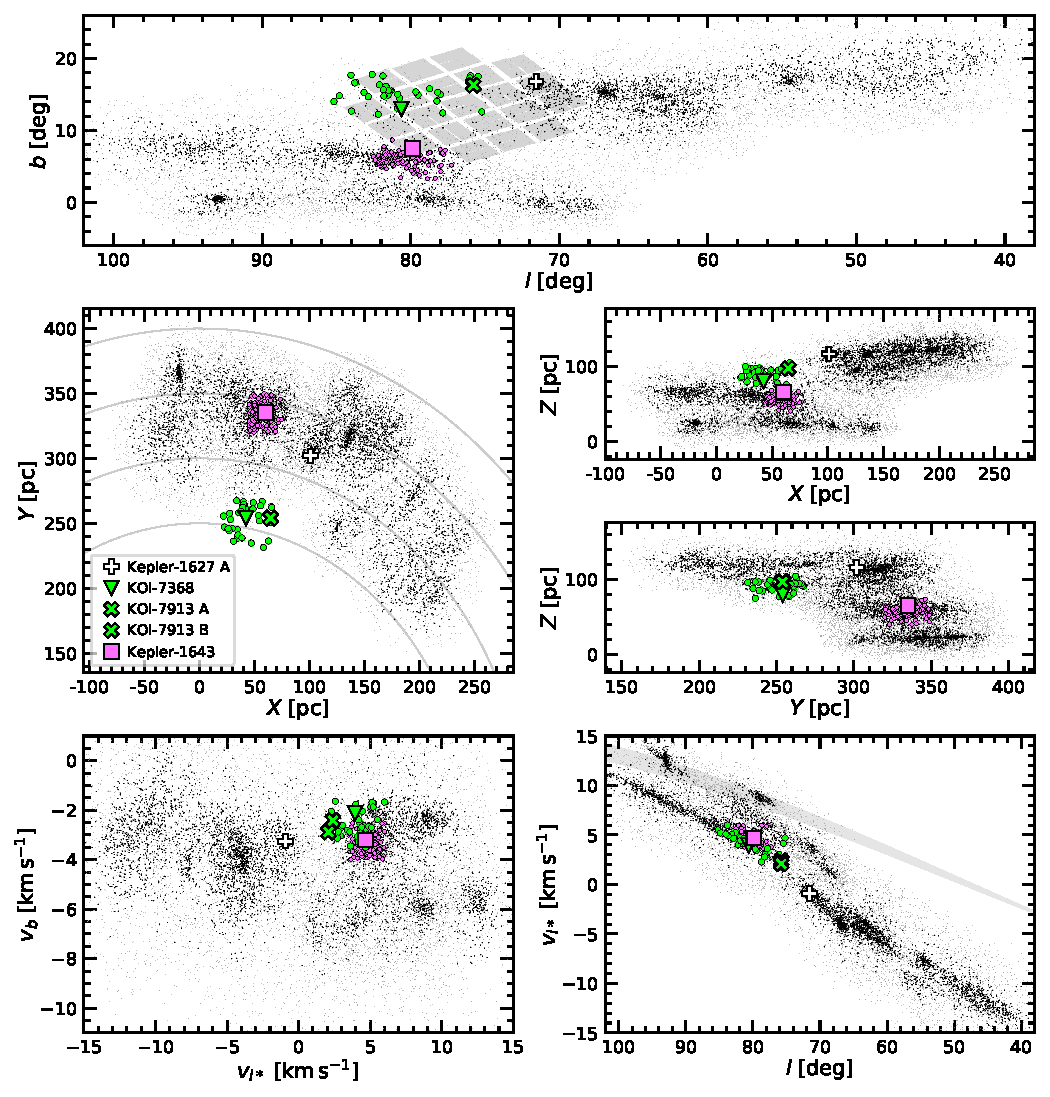
\includegraphics[width=0.99\textwidth]{f1.pdf}
	\end{center}
	\vspace{-0.7cm}
	\caption{
    {\bf Galactic positions  and tangential velocities of stars in the
    complex.}  {\bf This is a placeholder before we get real kinematics.}
    Sub-clusters include the $\delta$ Lyr cluster, RSG-5, and the
    worryingly diffuse ``CH-2''.
		\label{fig:XYZvtang}
	}
\end{figure*}

\subsection{Selecting Cluster Members}
\label{sec:kinematicselection}

\begin{figure*}[tp]
	\begin{center}
		\leavevmode
		\subfloat{
			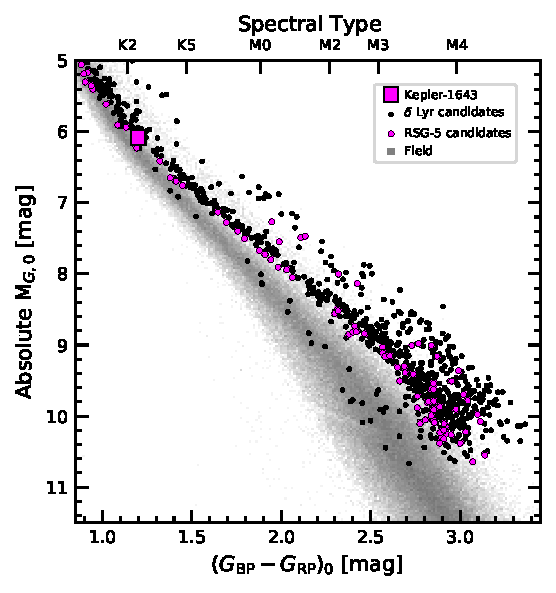
\includegraphics[width=0.49\textwidth]{f2a.pdf}
			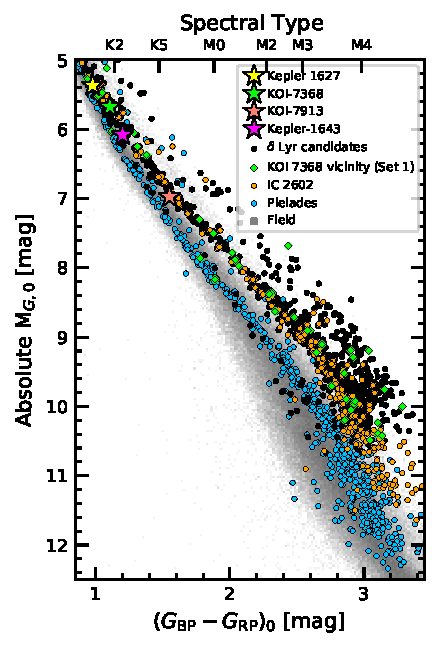
\includegraphics[width=0.469\textwidth]{f2b.pdf}
		}
		
		\vspace{-0.6cm}
		\subfloat{
			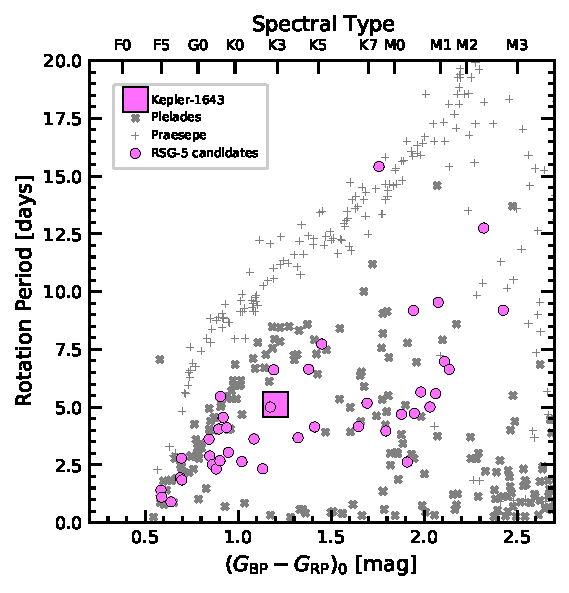
\includegraphics[width=0.49\textwidth]{f2c.pdf}
			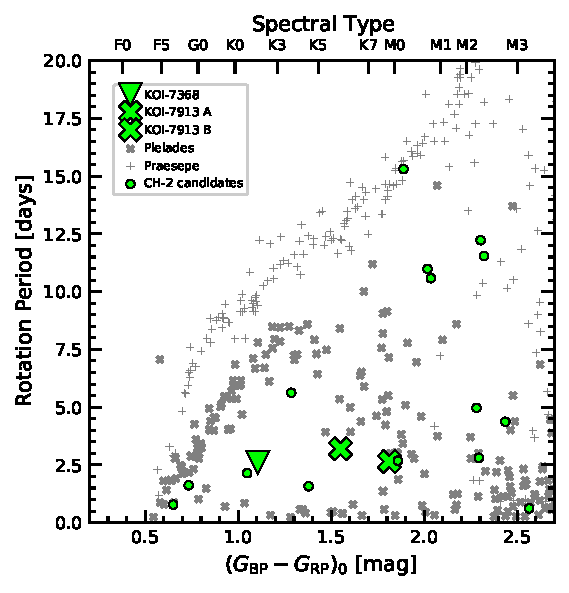
\includegraphics[width=0.49\textwidth]{f2d.pdf}
		}
	\end{center}
	\vspace{-0.7cm}
	\caption{
		{\bf The \cn\ is \clusterage\ old.} 
    The top row shows CAMDs.  Left shows CH-2, right shows RSG-5.
    The bottom left shows gyro (and is a {\bf place-holder since we might want to add CH-2 and RSG5}).
    The bottom right shows lithium (black points are NGC2547 and
    IC2602 from Randich+18 and probably are not believable at the red
    end; for Kepler-1643 I'm less confident, but it might be tied to the ``slow'' rotation period -- this is why we need RSG5 rotation periods).
    Also, we might want an
    H-alpha plot?).
		\label{fig:age}
	}
\end{figure*}

\subsection{The Cluster's Age}
\label{sec:clusterage}

\subsubsection{Color-Absolute Magnitude Diagram}
\label{sec:camd}

\subsubsection{Stellar Rotation Periods}

\section{The Stars}
\label{sec:stars}

\subsection{Kepler\,1627A}
\subsection{Kepler\,1643}
\subsection{KOI-7368}
\subsection{KOI-7913}
Is a binary.

\section{The Planets}
\label{sec:planet}

\begin{figure*}[tp]
	\begin{center}
		\leavevmode
		\subfloat{
			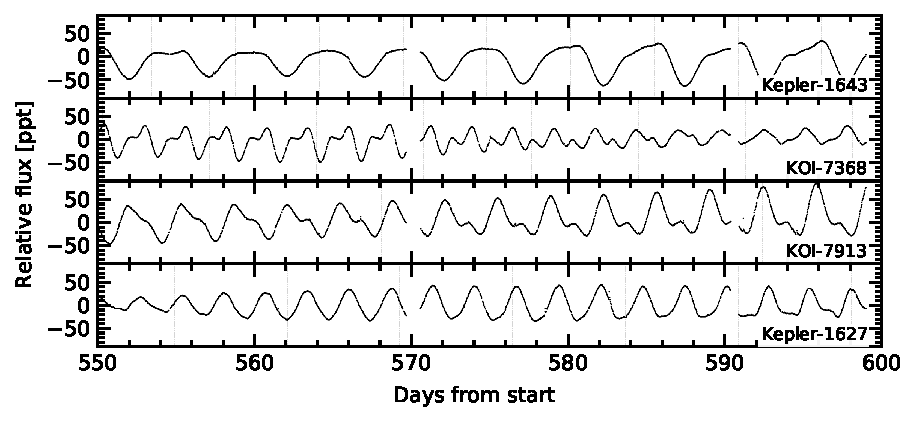
\includegraphics[width=0.99\textwidth]{f3e.pdf}
		}
		\vspace{-0.4cm}

		\subfloat{
			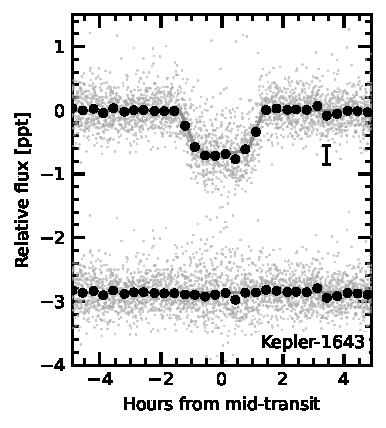
\includegraphics[width=0.47\textwidth]{f3a.pdf}
			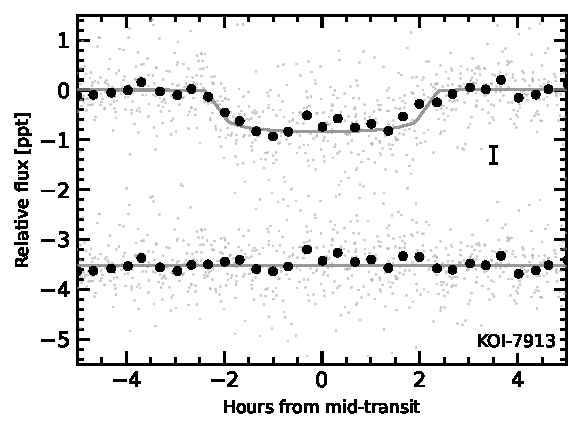
\includegraphics[width=0.47\textwidth]{f3b.pdf}
		}
		\vspace{-1.45cm}
	
		\subfloat{
			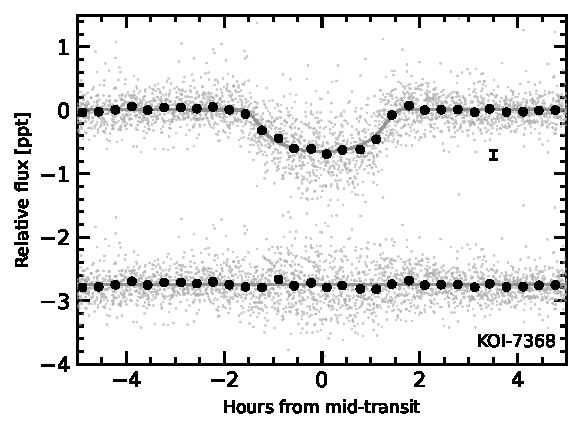
\includegraphics[width=0.47\textwidth]{f3c.pdf}
			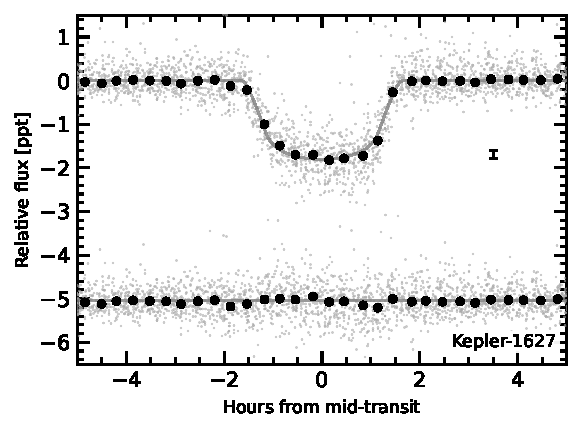
\includegraphics[width=0.47\textwidth]{f3d.pdf}
		}
	\end{center}
	\vspace{-0.7cm}
	\caption{
		{\bf Raw and processed light curves for the objects of
    interest.} Top: raw.  Bottom: processed.
    The increased scatter during transit is likely due to starspot
    crossing events.  KOI-7913 is janky, but P=24 days.
		\label{fig:planets}
	}
\end{figure*}


\section{Discussion \& Conclusions}
\label{sec:conc}

\begin{figure*}[!t]
	\begin{center}
		\leavevmode
		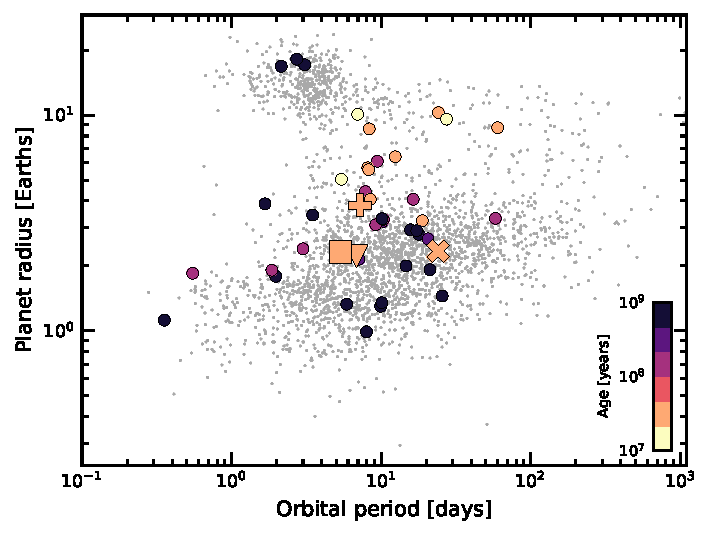
\includegraphics[width=0.9\textwidth]{f4.pdf}
	\end{center}
	\vspace{-0.7cm}
	\caption{
    %    namelist = ['Kepler-1627 A', 'KOI-7368', 'KOI-7913 A', 'KOI-7913 B', 'Kepler-1643']
    %    markers = ['P', 'v', 'X', 'X', 's']
		{\bf Radii, orbital periods, and ages of transiting exoplanets}.
		Planets younger than a gigayear with ${\rm \tau}/\sigma_{\tau} >
		3$ are emphasized, where $\tau$ is the age and $\sigma_{\tau}$ is
    its uncertainty. Kepler-1627 (+), KOI-7368 (down-triangle),
    KOI-7913 (X), Kepler-1643 (diamond).  The large sizes of
		the youngest transiting planets could be explained by their
		primordial atmospheres not yet having evaporated; direct
		measurements of the atmospheric outflows or planetary masses would
		help to confirm this expectation.  Selection effects may also be
		important.  Parameters are from the NASA Exoplanet Archive (2022
		Feb 27).
		\label{fig:rp_period_age}
	}
\end{figure*}


%%%%%%%%%%%%%%%%%%%%%%%%%%%%%%%%%%%%%%%%%%%%%%%%%%%%%%%%%%%%%%%%%%%%%%%%%%%%%%%


%\clearpage
\acknowledgements
\raggedbottom
%
L.G.B{.} acknowledges support from the TESS GI Program (NASA grants
80NSSC19K0386 and 80NSSC19K1728) and the Heising-Simons Foundation (51 Pegasi~b
Fellowship).
% programs G011103 and G022117, through 
%
%
%FIXME
Keck/NIRC2 imaging was acquired by program 2015A/N301N2L
(PI: A.~Kraus). % and 2019A/N069 (PI: E.~Petigura).
%
% ACKNOWLEDGE PFS / CAMPANAS.
%
This paper also includes data collected by the TESS mission, which are
publicly available from the Mikulski Archive for Space Telescopes
(MAST).
%
Funding for the TESS mission is provided by NASA's Science Mission
directorate.
%
We thank the TESS Architects (G.~Ricker, R.~Vanderspek, D.~Latham,
S.~Seager, J.~Jenkins) and the many TESS team members for their
efforts to make the mission a continued success.
%
%
%This study was based in part on observations at Cerro Tololo
%Inter-American Observatory at NSF's NOIRLab (NOIRLab Prop{.} ID
%2020A-0146; 2020B-0029 PI: Bouma), which is managed by the
%Association of Universities for Research in Astronomy (AURA) under a
%cooperative agreement with the National Science Foundation.
%
%
%Finally, this research has made use of the Keck Observatory Archive (KOA),
%which is operated by the W. M. Keck Observatory and the NASA Exoplanet
%Science Institute (NExScI), under contract with the National
%Aeronautics and Space Administration.
Finally, we also thank the Keck Observatory staff for their support of
HIRES and remote observing.  We recognize the importance that the
summit of Maunakea has within the indigenous Hawaiian community, and
are deeply grateful to have the opportunity to conduct observations
from this mountain.
%
% The Digitized Sky Survey was produced at the Space Telescope Science
% Institute under U.S. Government grant NAG W-2166.
% Figure~\ref{fig:scene} is based on photographic data obtained using
% the Oschin Schmidt Telescope on Palomar Mountain.
%

% %
% This research made use of the NASA Exoplanet Archive, which is
% operated by the California Institute of Technology, under contract
% with the National Aeronautics and Space Administration under the
% Exoplanet Exploration Program.
% %

% Resources supporting this work were provided by the NASA High-End
% Computing (HEC) Program through the NASA Advanced Supercomputing (NAS)
% Division at Ames Research Center for the production of the SPOC data
% products.
%

% A.J.\ and R.B.\ acknowledge support from project IC120009 ``Millennium
% Institute of Astrophysics (MAS)'' of the Millenium Science Initiative,
% Chilean Ministry of Economy. A.J.\ acknowledges additional support
% from FONDECYT project 1171208.  J.I.V\ acknowledges support from
% CONICYT-PFCHA/Doctorado Nacional-21191829.  R.B.\ acknowledges support
% from FONDECYT Post-doctoral Fellowship Project 3180246.
% %
% C.T.\ and C.B\ acknowledge support from Australian Research Council
% grants LE150100087, LE160100014, LE180100165, DP170103491 and
% DP190103688.
% %
% C.Z.\ is supported by a Dunlap Fellowship at the Dunlap Institute for
% Astronomy \& Astrophysics, funded through an endowment established by
% the Dunlap family and the University of Toronto.
% %
% D.D.\ acknowledges support through the TESS Guest Investigator Program
% Grant 80NSSC19K1727.
%
%
%
% %
% Based on observations obtained at the Gemini Observatory, which is
% operated by the Association of Universities for Research in Astronomy,
% Inc., under a cooperative agreement with the NSF on behalf of the
% Gemini partnership: the National Science Foundation (United States),
% National Research Council (Canada), CONICYT (Chile), Ministerio de
% Ciencia, Tecnolog\'{i}a e Innovaci\'{o}n Productiva (Argentina),
% Minist\'{e}rio da Ci\^{e}ncia, Tecnologia e Inova\c{c}\~{a}o (Brazil),
% and Korea Astronomy and Space Science Institute (Republic of Korea).
% %
% Observations in the paper made use of the High-Resolution Imaging
% instrument Zorro at Gemini-South. Zorro was funded by the NASA
% Exoplanet Exploration Program and built at the NASA Ames Research
% Center by Steve B. Howell, Nic Scott, Elliott P. Horch, and Emmett
% Quigley.
% %
% This research has made use of the VizieR catalogue access tool, CDS,
% Strasbourg, France. The original description of the VizieR service was
% published in A\&AS 143, 23.
% %
% This work has made use of data from the European Space Agency (ESA)
% mission {\it Gaia} (\url{https://www.cosmos.esa.int/gaia}), processed
% by the {\it Gaia} Data Processing and Analysis Consortium (DPAC,
% \url{https://www.cosmos.esa.int/web/gaia/dpac/consortium}). Funding
% for the DPAC has been provided by national institutions, in particular
% the institutions participating in the {\it Gaia} Multilateral
% Agreement.
%
% (Some of) The data presented herein were obtained at the W. M. Keck
% Observatory, which is operated as a scientific partnership among the
% California Institute of Technology, the University of California and
% the National Aeronautics and Space Administration. The Observatory was
% made possible by the generous financial support of the W. M. Keck
% Foundation.
% The authors wish to recognize and acknowledge the very significant
% cultural role and reverence that the summit of Maunakea has always had
% within the indigenous Hawaiian community.  We are most fortunate to
% have the opportunity to conduct observations from this mountain.
%
% \newline
%

\software{
  %\texttt{arviz} \citep{arviz_2019},
  %\texttt{altaipony} \citep{ilin_flares_2021},
  \texttt{astrobase} \citep{bhatti_astrobase_2018},
  %\texttt{astroplan} \citep{astroplan2018},
	%\texttt{AstroImageJ} \citep{collins_astroimagej_2017},
  \texttt{astropy} \citep{astropy_2018},
  \texttt{astroquery} \citep{astroquery_2018},
  %\texttt{BATMAN} \citep{kreidberg_batman_2015},
  %\texttt{ceres} \citep{brahm_2017_ceres},
  %\texttt{cdips-pipeline} \citep{bhatti_cdips-pipeline_2019},
  \texttt{corner} \citep{corner_2016},
  %\texttt{emcee} \citep{foreman-mackey_emcee_2013},
  \texttt{exoplanet} \citep{exoplanet:exoplanet}, and its
  dependencies \citep{exoplanet:agol20, exoplanet:kipping13, exoplanet:luger18,
   	exoplanet:theano},
	%\texttt{gala} \citep{gala,PriceWhelan_2017_gala_zenodo},
	%\texttt{IDL Astronomy User's Library} \citep{landsman_1995},
  %\texttt{IPython} \citep{perez_2007},
	%\texttt{isochrones} \citep{morton_2015_isochrones},
	%\texttt{lightkurve} \citep{lightkurve_2018},
  %\texttt{matplotlib} \citep{hunter_matplotlib_2007}, 
  %\texttt{MESA} \citep{paxton_modules_2011,paxton_modules_2013,paxton_modules_2015}
  %\texttt{numpy} \citep{walt_numpy_2011}, 
  %\texttt{pandas} \citep{mckinney-proc-scipy-2010},
  %\texttt{pyGAM} \citep{serven_pygam_2018_1476122},
  \texttt{PyMC3} \citep{salvatier_2016_PyMC3},
  %\texttt{radvel} \citep{fulton_radvel_2018},
  %\texttt{scikit-learn} \citep{scikit-learn},
  \texttt{scipy} \citep{jones_scipy_2001},
  %\texttt{TESS-point}  \citep{burke_2020},
  %\texttt{tesscut} \citep{brasseur_astrocut_2019},
	%\texttt{VESPA} \citep{morton_efficient_2012,vespa_2015},
  %\texttt{webplotdigitzer} \citep{rohatgi_2019},
  %\texttt{wotan} \citep{hippke_wotan_2019}.
}
\ 

\facilities{
 	{\it Astrometry}:
 	Gaia \citep{gaia_collaboration_gaia_2018,gaia_collaboration_2021_edr3}.
 	{\it Imaging}:
    Second Generation Digitized Sky Survey. %,
    %SOAR~(HRCam; \citealt{tokovinin_ten_2018}).
 	Keck:II~(NIRC2; \url{www2.keck.hawaii.edu/inst/nirc2}).
 	%Gemini:South~(Zorro; \citealt{scott_nessi_2018}.
 	%Gemini:North~(`Alopeke; \citealt{scott_nessi_2018,scott_twin_2021}.
 	{\it Spectroscopy}:
	%CTIO1.5$\,$m~(CHIRON; \citealt{tokovinin_chironfiber_2013}),
  %PFS ({\bf CITE}),
	Tillinghast:1.5m~(TRES; \citealt{furesz_tres_2008}).
  %MPG2.2$\,$m~(FEROS; \citealt{kaufer_commissioning_1999}),
	%AAT~(Veloce; \citealt{gilbert_veloce_2018}).
	%AAT~(HERMES; \citealt{lewis_2002_hermers_2df,sheinis_2015_hermes}),
 	Keck:I~(HIRES; \citealt{vogt_hires_1994}).
 	%VLT:Kueyen~(FLAMES; \citealt{pasquini_2002}).
% 	Euler1.2m~(CORALIE),
% 	ESO:3.6m~(HARPS; \citealt{mayor_setting_2003}).
 	{\it Photometry}:
%	  ASTEP:0.40$\,$m (ASTEP400),
% 	CTIO:1.0m (Y4KCam),
% 	Danish 1.54m Telescope,
%	  El Sauce:0.356$\,$m,
% 	Elizabeth 1.0m at SAAO,
% 	Euler1.2m (EulerCam),
	  Kepler \citep{borucki_kepler_2010},
% 	Magellan:Baade (MagIC),
% 	Max Planck:2.2m	(GROND; \citealt{greiner_grond7-channel_2008})
%   MuSCAT3 \citep{Narita_2020},
% 	NTT,
% 	SOAR (SOI),
 	  TESS \citep{ricker_transiting_2015}.
% 	TRAPPIST \citep{jehin_trappist_2011},
% 	VLT:Antu (FORS2).
}

% \begin{table*}
\scriptsize
\setlength{\tabcolsep}{2pt}
\centering
\caption{Literature and Measured Properties for Kepler$\,$1627}
\label{tab:starparams}
%\tablenum{2}
\begin{tabular}{llcc}
  \hline
  \hline
Primary Star\dotfill & \\
\multicolumn{3}{c}{TIC 120105470} \\
\multicolumn{3}{c}{GAIADR2$^\dagger$ 2103737241426734336} \\
\hline
\hline
Parameter & Description & Value & Source\\
\hline 
$\alpha_{J2015.5}$\dotfill	&Right Ascension (hh:mm:ss)\dotfill & 18:56:13.6 & 1	\\
$\delta_{J2015.5}$\dotfill	&Declination (dd:mm:ss)\dotfill & +41:34:36.22 & 1	\\
%
V\dotfill			&Johnson V mag.\dotfill & 13.11 $\pm$ 0.08		& 2	\\
${\rm G}$\dotfill     & Gaia $G$ mag.\dotfill     & 13.02$\pm$0.02 & 1\\
$G_{\rm BP}$\dotfill     & Gaia $BP$ mag.\dotfill     & 13.43$\pm$0.02 & 1\\
$G_{\rm RP}$\dotfill     & Gaia $RP$ mag.\dotfill     & 12.44$\pm$0.02 & 1\\
${\rm T}$\dotfill     & TESS $T$ mag.\dotfill     & 12.53$\pm$0.02 & 2\\
J\dotfill			& 2MASS J mag.\dotfill & 11.69  $\pm$ 0.02	& 3	\\
H\dotfill			& 2MASS H mag.\dotfill & 11.30 $\pm$ 0.02	    &  3	\\
K$_{\rm S}$\dotfill			& 2MASS ${\rm K_S}$ mag.\dotfill & 11.19 $\pm$ 0.02 &  3	\\
%
$\pi$\dotfill & Gaia EDR3 parallax (mas) \dotfill & 3.009 $\pm$ 0.032 &  1 \\
$d$\dotfill & Distance (pc)\dotfill & $329.5 \pm 3.5$ & 1, 4 \\
$\mu_{\alpha}$\dotfill		& Gaia EDR3 proper motion\dotfill & 1.716 $\pm$ 0.034 & 1 \\
                    & \hspace{3pt} in RA (mas yr$^{-1}$)	&  \\
$\mu_{\delta}$\dotfill		& Gaia EDR3 proper motion\dotfill 	&  -1.315 $\pm$ 0.034 &  1 \\
                    & \hspace{3pt} in DEC (mas yr$^{-1}$) &  \\
RUWE\dotfill		& Gaia EDR3 renormalized\dotfill 	&  2.899 &  1 \\
                    & \hspace{3pt} unit weight error &  \\
RV\dotfill & Systemic radial \hspace{9pt}\dotfill  & $-16.7 \pm 1.0$ & 5 \\
                    & \hspace{3pt} velocity (\kms)  & \\
%
Spec. Type\dotfill & Spectral Type\dotfill & 	G8V & 5 \\
$v\sin{i_\star}$\dotfill &  Rotational velocity$^*$ (\kms) \hspace{9pt}\dotfill &  18.9 $\pm$ 1.0 & 5 \\
Li EW\dotfill & 6708\AA\ Equiv{.} Width (m\AA) \dotfill & $233^{+5}_{-7}$  & 5 \\
$T_{\rm eff}$\dotfill &  Effective Temperature (K) \hspace{9pt}\dotfill & 5505 $\pm$ 60 &  6  \\
$\log{g_{\star}}$\dotfill &  Surface Gravity (cgs)\hspace{9pt}\dotfill &  4.53 $\pm$ 0.05  &  6 \\
$R_\star$\dotfill & Stellar radius ($R_\odot$)\dotfill & 0.881$\pm$0.018 & 6 \\
$M_\star$\dotfill & Stellar mass ($R_\odot$)\dotfill & 0.953$\pm$0.019 & 6 \\
$A_{\rm V}$\dotfill & Interstellar reddening (mag)\dotfill & 0.2 $\pm$ 0.1 & 6 \\
${\rm [Fe/H]}$\dotfill &   Metallicity\dotfill & 0.1 $\pm$ 0.1 & 6 \\
%
$P_{\rm rot}$\dotfill & Rotation period (d)\dotfill & $2.642\pm 0.042$  & 7 \\
Age & Adopted stellar age (Myr)\dotfill & $38^{+6}_{-5}$  &  8 \\
%
\hline 
%
$\Delta m_{832}$ & Mag difference (`Alopeke 832\,nm)\dotfill & $3.14 \pm 0.04$ & 9 \\
$\theta_{\rm B}$ & Position angle (deg)\dotfill & $91.9 \pm 0.7$ & 9 \\
$\rho_{\rm B}$ & Apparent separation of \dotfill & $0.164 \pm 0.010$ &  9 \\
                    & \hspace{3pt} primary and secondary (as) &  \\
$\rho_{\rm B}$ & Apparent separation of \dotfill & $53 \pm 4$ &  1,4,9 \\
                    & \hspace{3pt} primary and secondary (AU) &  \\
$\Delta m_{K'}$ & Mag difference (NIRC2 $K'$)\dotfill & $2.37 \pm 0.02$ & 10 \\
$\theta_{\rm B}$ & Position angle (deg)\dotfill & $95.9 \pm 0.5$ & 10 \\
$\rho_{\rm B}$ & Apparent separation of \dotfill & $0.1739 \pm 0.0017$ &  10 \\
                    & \hspace{3pt} primary and secondary (as) &  \\
%
\hline
\end{tabular}
\begin{flushleft}
 \footnotesize{ \textsc{NOTE}---
 $^\dagger$ The GAIADR2 and GAIAEDR3 identifiers for Kepler 1627A are identical.  The secondary
 is not resolved in the Gaia point source catalog.
 $^*$ Given only $v\sin i$ and $2\piR_\star/P_{\rm rot}$, $\cos i=0.11^{+0.11}_{-0.08}$.
Provenances are:
$^1$\citet{gaia_collaboration_2021_edr3},
$^2$\citet{stassun_TIC8_2019},
$^3$\citet{skrutskie_tmass_2006},
$^4$\citet{Lindegren_2021_offset},
$^5$HIRES spectra and \citet{yee_SM_2017},
$^6$Cluster isochrone (MIST adopted; PARSEC compared for quoted
  uncertainty),
$^7$Kepler light curve,
$^8$Pre-main-sequence CAMD interpolation (Section~\ref{sec:camd}),
$^9$`Alopeke imaging 2021 June 24 \citep{scott_twin_2021},
$^{10}$NIRC2 imaging 2015 July 22.
}
\end{flushleft}
\vspace{-0.5cm}
\end{table*}

% % Table of best fit parameters
%\startlongtable
\begin{deluxetable*}{lllrrrrrrr}
%
  \tablecaption{ Priors and posteriors for the transit and stellar
  variability model fitted to the long-cadence Kepler 1627b
  photometric timeseries.}
\label{tab:posterior}
%
\tabletypesize{\scriptsize}
%\tabletypesize{\small}
%
%\tablenum{2}
%
\tablehead{
  \colhead{Param.} & 
  \colhead{Unit} &
  \colhead{Prior} & 
  \colhead{Median} & 
  \colhead{Mean} & 
  \colhead{Std{.} Dev.} &
  \colhead{3\%} &
  \colhead{97\%} &
  \colhead{ESS} &
  \colhead{$\hat{R}-1$}
}

%/Users/luke/Dropbox/proj/rudolf/results/run_RotStochGPtransit/Kepler_1627_RotStochGPtransit_posteriortable.tex
\startdata
{\it Sampled} & & & & & & & & & \\
\hline
$P$ & d & $\mathcal{N}(7.20281; 0.01000)$ & 7.2028035 & 7.2028033 & 0.0000073 & 7.2027893 & 7.2028171 & 1910.5903732 & 0.0035905 \\
$t_0^{(1)}$ & d & $\mathcal{N}(120.79053; 0.02000)$ & 120.790504 & 120.790505 & 0.0009438 & 120.7886867 & 120.7922431 & 1564.1105056 & 0.0003213 \\
$\log R_{\rm p}/R_\star$ & -- & $\mathcal{U}(-4.605; 0.000)$ & -3.33523 & -3.33569 & 0.06618 & -3.45772 & -3.21617 & 1173.56574 & 0.00310 \\
$b$ & -- & $\mathcal{U}(0; 1+R_{\mathrm{p}}/R_\star)$ & 0.3971 & 0.3886 & 0.2070 & 0.0204 & 0.7289 & 378.9528 & 0.0177 \\
$u_1$ & -- & \citet{exoplanet:kipping13} & 0.28 & 0.30 & 0.179 & 0.002 & 0.603 & 1161.95 & 0.005 \\
$u_2$ & -- & \citet{exoplanet:kipping13} & 0.425 & 0.381 & 0.314 & -0.197 & 0.912 & 900.884 & 0.002 \\
$R_\star$ & $R_\odot$ & $\mathcal{T}(0.910; 0.052)$ & 0.911 & 0.910 & 0.051 & 0.814 & 1.004 & 2265.830 & -0.001 \\
$\log g$ & cgs & $\mathcal{N}(4.600; 0.100)$ & 4.604 & 4.601 & 0.094 & 4.417 & 4.769 & 923.943 & 0. \\
$\langle f \rangle$ & -- & $\mathcal{N}(0.500; 0.100)$ & 0.4999 & 0.4999 & 0.0003 & 0.4993 & 0.5005 & 2964.6676 & 0.0013 \\
$e^{(2)}$ & -- & \citet{vaneylen19} & 0.127 & 0.168 & 0.147 & 0. & 0.446 & 518.492 & 0.004 \\
$\omega$ & rad & $\mathcal{U}(0.000; 6.283)$ & -0.235 & -0.170 & 1.867 & -2.879 & 3.132 & 1212.260 & 0.006 \\
$\log \sigma_f$ & -- & $\mathcal{N}(\log\langle \sigma_f \rangle; 2.000)$ & -8.016 & -8.016 & 0.008 & -8.031 & -8.001 & 2224.427 & -0. \\
$\rho$ & d & $\mathcal{U}(1.000; 10.000)$ & 2.953 & 2.955 & 0.096 & 2.777 & 3.131 & 1936.492 & 0. \\
$\sigma$ & d$^{-1}$ & $\mathrm{InvGamma}(1.000; 5.000)$ & 0.013 & 0.013 & 0.001 & 0.012 & 0.014 & 2155.687 & -0. \\
$\sigma_{\mathrm{rot}}$ & d$^{-1}$ & $\mathrm{InvGamma}(1.000; 5.000)$ & 0.897 & 0.933 & 0.222 & 0.552 & 1.316 & 2147.324 & 0.003 \\
$\log P_{\mathrm{rot}}$ & $\log (\mathrm{d})$ & $\mathcal{N}(0.958; 0.020)$ & 0.964 & 0.964 & 0.001 & 0.963 & 0.966 & 2486.029 & 0. \\
$\log Q_0$ & -- & $\mathcal{N}(0.000; 2.000)$ & 12.935 & 12.960 & 0.454 & 12.157 & 13.857 & 2126.581 & 0.004 \\
$\log \mathrm{d}Q$ & -- & $\mathcal{N}(0.000; 2.000)$ & 0.029 & 0.021 & 2.032 & -3.785 & 3.780 & 1755.941 & 0. \\
$f$ & -- & $\mathcal{U}(0.100; 1.000)$ & 0.111 & 0.113 & 0.010 & 0.1 & 0.130 & 1253.358 & -0.0 \\
\hline
{\it Derived} & & & & & & & & & \\
\hline
$R_{\rm p}/R_\star$ & -- & -- & 0.036 & 0.036 & 0.002 & 0.031 & 0.040 & 1173.566 & 0.003 \\
$\rho_\star$ & g$\ $cm$^{-3}$ & -- & 2.27 & 2.312 & 0.516 & 1.408 & 3.272 & 910.746 & 0.001 \\
$R_{\rm p}$ & $R_{\mathrm{Jup}}$ & -- & 0.316 & 0.317 & 0.037 & 0.251 & 0.386 & 1692.736 & 0.001 \\
$a/R_\star$ & -- & -- & 18.396 & 18.407 & 1.375 & 15.690 & 20.780 & 910.717 & 0.001 \\
$\cos i$ & -- & -- & 0.022 & 0.021 & 0.011 & 0.002 & 0.038 & 439.303 & 0.011 \\
$T_{14}$ & hr & -- & 2.822 & 2.823 & 0.057 & 2.710 & 2.917 & 1086.008 & 0.002 \\
$T_{13}$ & hr & -- & 2.578 & 2.566 & 0.083 & 2.430 & 2.714 & 590.630 & 0.011 \\
\enddata
%
\tablecomments{
  ESS refers to the number of effective samples.
  $\hat{R}$ is the Gelman-Rubin convergence diagnostic.
  Logarithms through this table are in base-$e$.
  $\mathcal{U}$ denotes a uniform distribution,
  $\mathcal{N}$ a normal distribution, and
  $\mathcal{T}$ a truncated normal bounded between zero and an upper limit much larger than the mean.
  (1) The ephemeris is in units of BJDTDB - 2454833.
  (2) The eccentricity vectors are sampled in the $(e\cos\omega,
  e\sin\omega)$ basis.
%
% (2) Uninformative quadratic limb-darkening prior from \citet{exoplanet:kipping13}, implemented by \citet{exoplanet:exoplanet}.
% The precision achieved in the ground-based data did not appear to
% necessitate using bandpass-dependent limb-darkening coefficients.
% For comparison, the \citet{claret_limb_2017} parameters for
% the appropriate $T_{\rm eff}$ and $\log g$ in TESS-band would have been 
% $(u_1, u_2) = (0.3249, 0.235)$.
%
% (2) Assuming an informative quadratic limb-darkening prior with
% values about those given for the appropriate $T_{\rm eff}$ and
% $\log g$ in TESS-band from \citet{claret_limb_2017}. The precision
% achieved in the ground-based data did not appear to necessitate using
% bandpass-dependent limb-darkening coefficients.
% (3) The second and third contact points do not exist for a grazing transit.
% {\it Notation}:
% $a_{ij;\mathrm{Instr}}$ denotes the $i^{\rm th}$ transit of a
% particular instrument, and the $j^{\rm th}$ polynomial detrending
% order.
}
\vspace{-0.3cm}
\end{deluxetable*}

% %% \begin{deluxetable}{} command tell LaTeX how many columns
%% there are and how to align them.
%\startlongtable
\begin{deluxetable*}{lll}
    
%% Keep a portrait orientation

%% Over-ride the default font size
%% Use Default (12pt)
\tabletypesize{\scriptsize}
%\tabletypesize{\small}

%% Use \tablewidth{?pt} to over-ride the default table width.
%% If you are unhappy with the default look at the end of the
%% *.log file to see what the default was set at before adjusting
%% this value.

%% This is the title of the table.
\tablecaption{Young, Age-dated, and Age-dateable Stars Within the
  Nearest Few Kiloparsecs ($\texttt{v0.5}$ of the CDIPS Target
  List).}
\label{tab:v05}

%% This command over-rides LaTeX's natural table count
%% and replaces it with this number.  LaTeX will increment 
%% all other tables after this table based on this number
%\tablenum{3}

%% The \tablehead gives provides the column headers.  It
%% is currently set up so that the column labels are on the
%% top line and the units surrounded by ()s are in the 
%% bottom line.  You may add more header information by writing
%% another line between these lines. For each column that requries
%% extra information be sure to include a \colhead{text} command
%% and remember to end any extra lines with \\ and include the 
%% correct number of &s.
\tablehead{
  \colhead{Parameter} &
  \colhead{Example Value} &
  \colhead{Description}
}

%% All data must appear between the \startdata and \enddata commands
%
% paste from
% /Users/luke/Dropbox/proj/rudolf/results/tables/v05_main_tableheader.tex
% via drivers/write_v05_main_tableheader.py
\startdata
         \texttt{source\_id} &                                         1709456705329541504 &                                             Gaia DR2 source identifier. \\
                 \texttt{ra} &                                                     247.826 &                                         Gaia DR2 right ascension [deg]. \\
                \texttt{dec} &                                                      79.789 &                                             Gaia DR2 declination [deg]. \\
           \texttt{parallax} &                                                      35.345 &                                                Gaia DR2 parallax [mas]. \\
    \texttt{parallax\_error} &                                                       0.028 &                                    Gaia DR2 parallax uncertainty [mas]. \\
               \texttt{pmra} &                                                      94.884 &     Gaia DR2 proper motion $\mu_\alpha \cos \delta$ [mas$\,$yr${^-1}$]. \\
              \texttt{pmdec} &                                                     -86.971 &                 Gaia DR2 proper motion $\mu_\delta$ [mas$\,$yr${^-1}$]. \\
 \texttt{phot\_g\_mean\_mag} &                                                        6.85 &                                                 Gaia DR2 $G$ magnitude. \\
\texttt{phot\_bp\_mean\_mag} &                                                       6.409 &                                     Gaia DR2 $G_\mathrm{BP}$ magnitude. \\
\texttt{phot\_rp\_mean\_mag} &                                                       7.189 &                                     Gaia DR2 $G_\mathrm{RP}$ magnitude. \\
            \texttt{cluster} &                 Uma,IR\_excess,NASAExoArchive\_ps\_20210506 &                                  Comma-separated cluster or group name. \\
                \texttt{age} &                                                nan,nan,9.48 & Comma-separated logarithm (base-10) of reported$^{\rm a}$ age in years. \\
          \texttt{mean\_age} &                                                        9.48 &                          Mean (ignoring NaNs) of $\texttt{age}$ column. \\
      \texttt{reference\_id} &      Ujjwal2020,CottenSong2016,NASAExoArchive\_ps\_20210506 &                          Comma-separted provenance of group membership. \\
 \texttt{reference\_bibcode} & 2020AJ....159..166U,2016ApJS..225...15C,2013PASP..125..989A &                  ADS bibcode corresponding to $\texttt{reference\_id}$. \\
\enddata

%% Include any \tablenotetext{key}{text}, \tablerefs{ref list},
%% or \tablecomments{text} between the \enddata and 
%% \end{deluxetable} commands

%% General table comment marker
\tablecomments{
Table~\ref{tab:v05} is
published in its entirety in a machine-readable format.   This table is a
concatenation of the studies listed in Table~\ref{tab:metadata}.
One entry is
shown for guidance regarding form and content. 
In this particular example, the star has a
cold Jupiter on a 16 year orbit, HD 150706b \citep{2012AA...545A..55B}.
An infrared excess has been reported \citep{CottenSong2016}, and the star was identified by \citet{Ujjwal2020} as a candidate UMa moving group
member ($\approx 400\,{\rm Myr}$; \citealt{mann_tess_2020}).
The star's RV activity and TESS rotation period corroborate its youth.
}
\vspace{-0.5cm}
\end{deluxetable*}

% %% \begin{deluxetable}{} command tell LaTeX how many columns
%% there are and how to align them.
%\startlongtable
\begin{deluxetable*}{lccc}
    
%% Keep a portrait orientation

%% Over-ride the default font size
%% Use Default (12pt)
\tabletypesize{\scriptsize}
%\tabletypesize{\small}
%\tabletypesize{\normal}

%% Use \tablewidth{?pt} to over-ride the default table width.
%% If you are unhappy with the default look at the end of the
%% *.log file to see what the default was set at before adjusting
%% this value.

%% This is the title of the table.
\tablecaption{Provenances of Young and Age-dateable Stars.}
\label{tab:metadata}

%% This command over-rides LaTeX's natural table count
%% and replaces it with this number.  LaTeX will increment 
%% all other tables after this table based on this number
%\tablenum{3}

%% The \tablehead gives provides the column headers.  It
%% is currently set up so that the column labels are on the
%% top line and the units surrounded by ()s are in the 
%% bottom line.  You may add more header information by writing
%% another line between these lines. For each column that requries
%% extra information be sure to include a \colhead{text} command
%% and remember to end any extra lines with \\ and include the 
%% correct number of &s.
\tablehead{
  \colhead{Reference} &
  \colhead{$N_{\rm Gaia}$} &
  \colhead{$N_{\rm Age}$} &
  \colhead{$N_{G_{\rm RP}<16}$}
}

%% All data must appear between the \startdata and \enddata commands
%
% paste from
% /Users/luke/Dropbox/proj/rudolf/results/tables/metadata_table_data.tex
% via drivers/write_metadata_table.py
\startdata
                           \citet{Kounkel2020}  &             987376 &            987376 &                775363 \\
                     \citet{CantatGaudin2020a}  &             433669 &            412671 &                269566 \\
                     \citet{CantatGaudin2018a}  &             399654 &            381837 &                246067 \\
                      \citet{KounkelCovey2019}  &             288370 &            288370 &                229506 \\
                     \citet{CantatGaudin2020b}  &             233369 &            227370 &                183974 \\
                           \citet{Zari2018} UMS &              86102 &                 0 &                 86102 \\
                  \citet{SIMBAD} $\texttt{Y*?}$ &              61432 &                 0 &                 45076 \\
                           \citet{Zari2018} PMS &              43719 &                 0 &                 38435 \\
\citet{GaiaCollaboration2018} $d>250\,{\rm pc}$ &              35506 &             31182 &                 18830 \\
                      \citet{CastroGinard2020}  &              33635 &             24834 &                 31662 \\
                              \citet{Kerr2021}  &              30518 &             25324 &                 27307 \\
                  \citet{SIMBAD} $\texttt{Y*O}$ &              28406 &                 0 &                 16205 \\
                        \citet{VillaVelez2018}  &              14459 &             14459 &                 13866 \\
                     \citet{CantatGaudin2019a}  &              11843 &             11843 &                  9246 \\
                        \citet{Damiani2019} PMS &              10839 &             10839 &                  9901 \\
                                \citet{Oh2017}  &              10379 &                 0 &                 10370 \\
                          \citet{Meingast2021}  &               7925 &              7925 &                  5878 \\
                 \citet{SIMBAD} $\texttt{pMS*}$ &               5901 &                 0 &                  3006 \\
\citet{GaiaCollaboration2018} $d<250\,{\rm pc}$ &               5378 &               817 &                  3968 \\
                           \citet{Kounkel2018}  &               5207 &              3740 &                  5207 \\
                        \citet{Ratzenbock2020}  &               4269 &              4269 &                  2662 \\
                  \citet{SIMBAD} $\texttt{TT*}$ &               4022 &                 0 &                  3344 \\
                        \citet{Damiani2019} UMS &               3598 &              3598 &                  3598 \\
                           \citet{Rizzuto2017}  &               3294 &              3294 &                  2757 \\
            \citet{NASAExoArchive_ps_20210506}  &               3107 &               868 &                  3098 \\
                              \citet{Tian2020}  &               1989 &              1989 &                  1394 \\
                           \citet{Goldman2018}  &               1844 &              1844 &                  1783 \\
                        \citet{CottenSong2016}  &               1695 &                 0 &                  1693 \\
                            \citet{Gagne2018a}  &               1429 &                 0 &                  1389 \\
             \citet{RoserSchilbach2020} Psc-Eri &               1387 &              1387 &                  1107 \\
            \citet{RoserSchilbach2020} Pleiades &               1245 &              1245 &                  1019 \\
                  \citet{SIMBAD} $\texttt{TT?}$ &               1198 &                 0 &                   853 \\
                            \citet{Gagne2018c}  &                914 &                 0 &                   913 \\
                          \citet{Pavlidou2021}  &                913 &               913 &                   504 \\
                            \citet{Gagne2018b}  &                692 &                 0 &                   692 \\
                            \citet{Ujjwal2020}  &                563 &                 0 &                   563 \\
                             \citet{Gagne2020}  &                566 &               566 &                   351 \\
                      \citet{EsplinLuhman2019}  &                377 &               443 &                   296 \\
                     \citet{Roccatagliata2020}  &                283 &               283 &                   232 \\
                          \citet{Meingast2019}  &                238 &               238 &                   238 \\
                 \citet{Furnkranz2019} Coma-Ber &                214 &               214 &                   213 \\
           \citet{Furnkranz2019} Neighbor Group &                177 &               177 &                   167 \\
                             \citet{Kraus2014}  &                145 &               145 &                   145 \\
\enddata

%% Include any \tablenotetext{key}{text}, \tablerefs{ref list},
%% or \tablecomments{text} between the \enddata and 
%% \end{deluxetable} commands

%% General table comment marker
\tablecomments{
Table~\ref{tab:metadata} describes the provenances for the young and
age-dateable stars in Table~\ref{tab:v06}.  $N_{\rm Gaia}$: number of
Gaia stars we parsed from the literature source.  $N_{\rm Age}$:
number of stars in the literature source with ages reported.
$N_{G_{\rm RP}<16}$: number of Gaia stars we parsed from the
literature source with either $G_{\rm RP}<16$, or a parallax S/N
exceeding 5 and a distance closer than 100\,pc.  The latter criterion
included a few hundred white dwarfs that would have otherwise been
neglected.  Some studies are listed multiple times if they contain
multiple tables.  \citet{SIMBAD} refers to the \texttt{SIMBAD}
database.
}
\vspace{-0.5cm}
\end{deluxetable*}


\clearpage
\bibliographystyle{yahapj}                            
\bibliography{bibliography} 

%\appendix
%\section{Young, Age-Dated, and Age-Dateable Star Compilation}
%\label{app:targetlist}


%\listofchanges
%\allauthors
\end{document}
